\subsection{Systembeschreibung}
Die Umsetzung der Wissenserwerbskomponente erfolgt am Beispiel von \textit{PaaSfinder}\footnote{{\label{foot:paasfinder}}https://paasfinder.org}, einem Expertensystem und Open-Source-Projekt im Bereich von \acf{PaaS}. Das Ziel des Systems besteht darin, zahlreiche PaaS-Anbieter (im Weiteren Vendors) vergleichbar zu machen. \textit{PaaSfinder} verf�gt bereits �ber eine umfangreiche Wissensdatenbank, die aufgrund der h�ufigen �nderungen im gegebenen Anwendungsbereich regelm��ig aktualisiert werden muss. Die Struktur von \textit{PaaSfinder} l�sst sich wie in Abbildung \ref{fig:paasfinder} beschreiben.
\begin{figure}[H] 
	\centering
	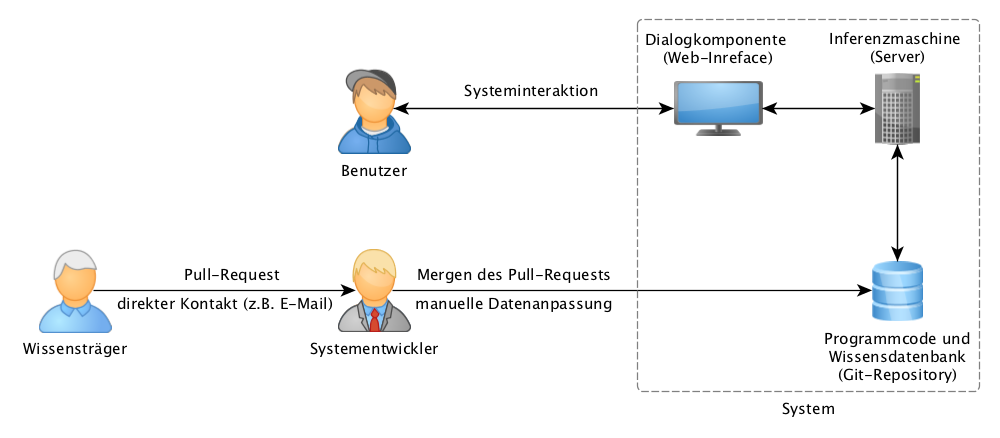
\includegraphics[width=0.9\textwidth]{images/paasfinder.png}
	\caption{Die Struktur von \textit{PaaSfinder}}
	\label{fig:paasfinder}
\end{figure} 
\textit{PaaSfinder} setzt sich aus dem Programmcode der Wissensdatenbank und der Webanwendung zusammen. Die Webanwendung wird wiederum auf einem Server betrieben. Ein Vendor wird in einem Profil\footnote{https://github.com/stefan-kolb/paas-profiles\#profile-specification} beschrieben, das wie folgt aufgebaut ist:
\begin{enumerate}
\item \textbf{General Properties}: allgemeine Eigenschaften des Vendors (z.B.\ Name, \acs{URL} oder \acs{URI}, Status, Typ etc.)
\item \textbf{Extensible}: generelle Erweiterungsm�glichkeit nach Kundenbedarf (z.B.\ spezielle Laufzeitumgebung)
\item \textbf{Pricing}: verf�gbare Preismodelle
\item \textbf{Quality of Service}: die Servicequalit�t (z.B.\ Verf�gbarkeit)
\item \textbf{Hosting}: Art der Bereitstellung (z.B.\ privat)
\item \textbf{Scaling}: Skalierbarkeit (z.B.\ Speichererweiterung)
\item \textbf{Runtimes}: unterst�tzte Laufzeitumgebungen (z.B.\ Java\footnote{https://java.com})
\item \textbf{Middleware} (z.B.\ Tomcat\footnote{https://tomcat.apache.org})
\item \textbf{Frameworks} (z.B.\ Play\footnote{https://www.playframework.com})
\item \textbf{Services} (z.B.\ Datenspeicher)
\item \textbf{Infrastructures} (z.B.\ Informationen zum Standort)
\end{enumerate}
Ein Vendor wird als \acs{JSON}\footnote{\label{foot:json}http://json.org}-Eintrag gespeichert. JSON ist ein Datenaustauschformat und basiert auf zwei Datenstrukturen: 
\begin{itemize}
\item \textit{Name/Wert Paar}, das ein Objekt darstellt (siehe Abbildung \ref{fig:json-object}).
\item \textit{Eine geordnete Liste von Werten (Array)}, die kein oder mehrere durch Komma getrennte Objekte enth�lt (siehe Abbildung \ref{fig:json-array}).
\end{itemize}
\begin{figure}[H] 
	\centering
	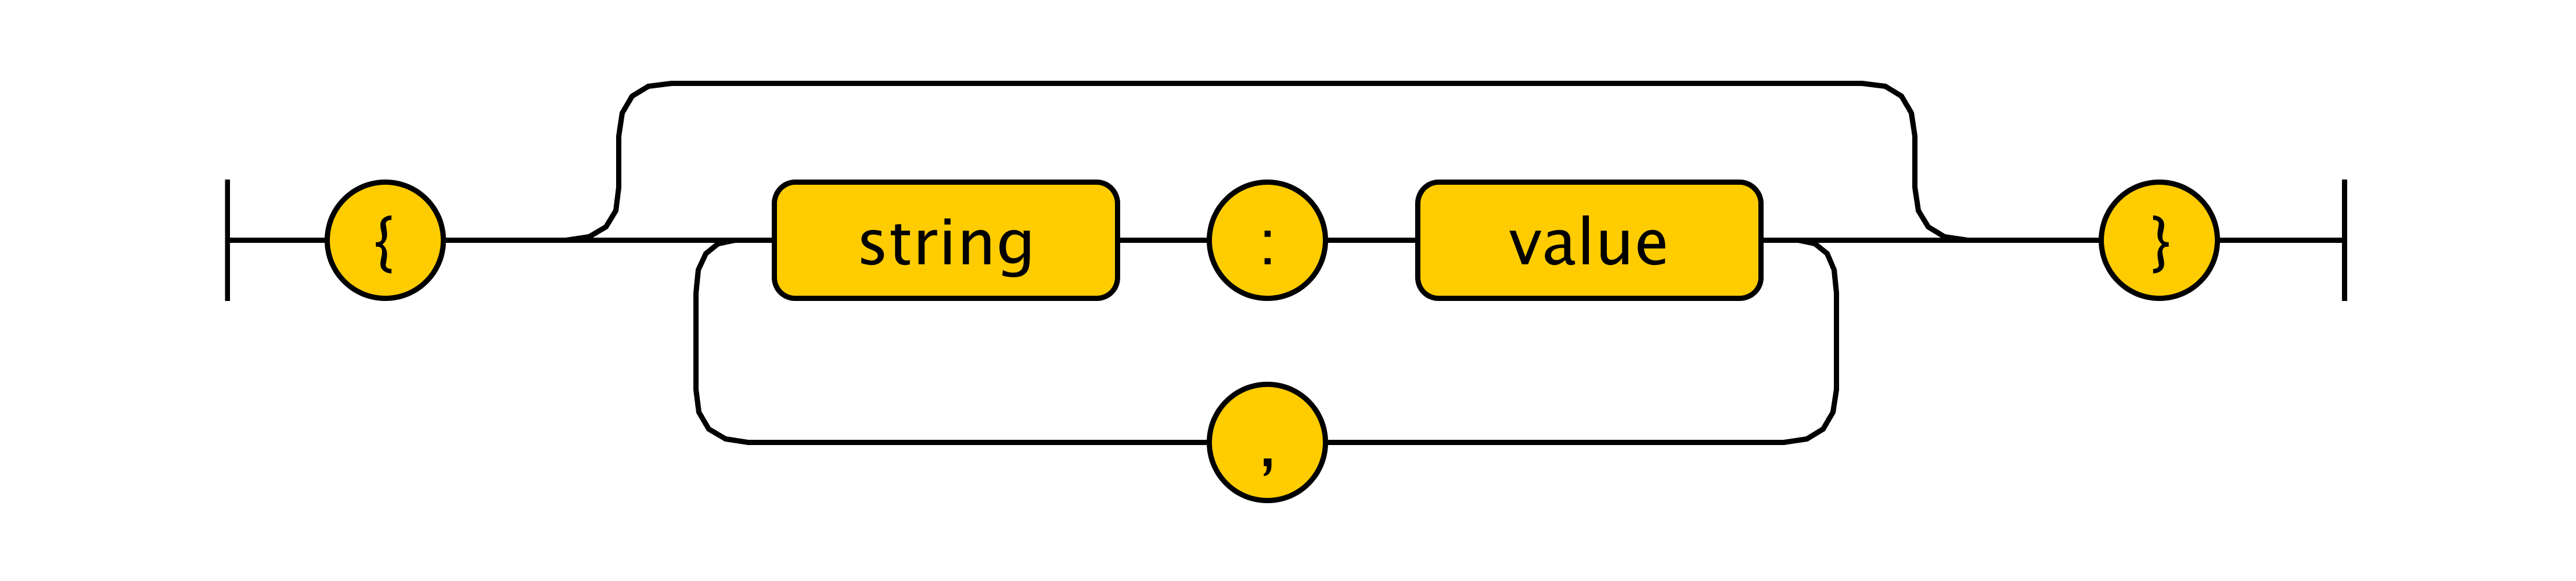
\includegraphics[width=0.85\textwidth]{images/json-object.png}
	\caption{JSON-Objekt Spezifikation}
	\label{fig:json-object}
\end{figure} 
\begin{figure}[H] 
	\centering
	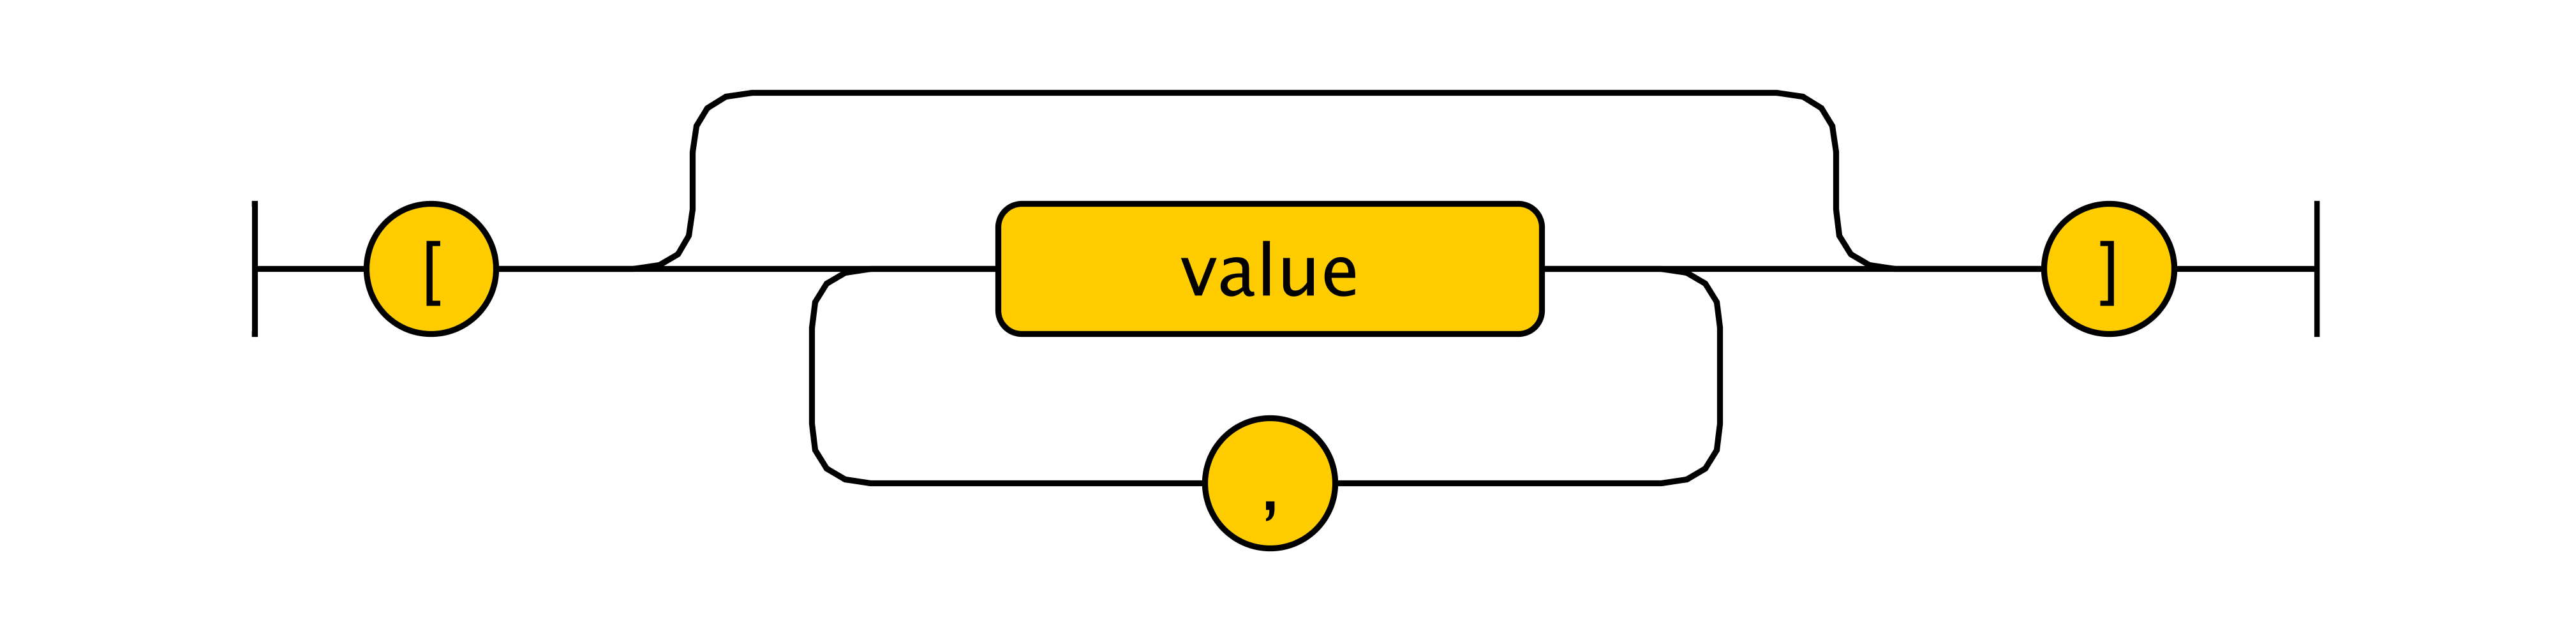
\includegraphics[width=0.75\textwidth]{images/json-array.png}
	\caption{JSON-Array Spezifikation}
	\label{fig:json-array}
\end{figure} 
Die Wissensdatenbank und der Programmcode von \textit{PaaSfinder} befinden sich in einem Git-Repository. Bei Git\footnote{https://git-scm.com} handelt es sich um eine Anwendung zur verteilten Projektverwaltung. Da \textit{PaaSfinder} ein Open-Source-Projekt ist, kann im Prinzip jeder die Wissensdatenbank erweitern bzw. modifizieren. Momentan kann das auf zwei Weisen erfolgen (siehe Abbildung \ref{fig:paasfinder}):
\begin{itemize}
\item \textit{Pull Request\footnote{https://git-scm.com/docs/git-request-pull}}
\item \textit{Direkter Kontakt mit dem Systementwickler} 
\end{itemize}
Beim Pull Request wird zuerst das gesamte Git-Repository lokal gespeichert. Danach werden �nderungen vorgenommen und anschlie�end eine Anfrage beim Projektmaster gestellt. Diese wird vom Projektmaster �berpr�ft und zugeh�rige �nderungen �bernommen (\glqq{}gemerged\grqq{}), falls keine Konflikte mit vorhandenen Daten vorliegen. Wenn der Wissenstr�ger mit dem Git-System nicht vertraut ist, kann direkter Kontakt (beispielsweise per E-Mail) mit dem Systementwickler aufgenommen werden. Die Daten werden dann manuell vom Systemverwalter in die Wissensbasis eingetragen.\\
Sowohl Pull Requests, als auch der Kontakt mit dem Systementwickler entsprechen dem direkten Wissenserwerb gem�� der Klassifikation in Kapitel \ref{subsec:Wissenserwerbskomponente}. Der Vorteil dabei ist, dass die Daten nicht manuell gesucht werden m�ssen, sondern direkt vom Wissenstr�ger stammen. Andererseits wird die Datenerfassung durch fehlende Git-Kenntnisse des Wissenstr�gers beschr�nkt. Um den direkten Wissenserwerb zu erleichtern, wird im weiteren Verlauf die Wissenstr�gerschnittstelle entwickelt, die es dem Wissenstr�ger erm�glicht, einen bestehenden Vendor zu aktualisieren. Nach dem erfolgreichen Absenden der �nderungen soll automatisch ein Pull Request erstellt werden. 